\documentclass[12pt, a4paper]{article}

\usepackage{xltxtra} % XeLaTex

\setromanfont{Liberation Sans} %Fonts setup
\setsansfont{Liberation Sans}
\setmonofont{DejaVu Sans Mono}

\usepackage{geometry}
\geometry{verbose,a4paper,tmargin=2cm,bmargin=2cm,lmargin=3.5cm,rmargin=1cm}

\usepackage{polyglossia} %Languages
\setmainlanguage{russian}
\setotherlanguage{english}

\PolyglossiaSetup{russian}{indentfirst=true} %Indentation
\parindent = 1cm

\usepackage{setspace}
\onehalfspacing
\hyphenpenalty=10000
\tolerance=1
\emergencystretch=1000

\usepackage{titlesec} %Настройка заголовков
\newcommand{\sectionbreak}{\clearpage}
\newcommand{\anonsection}[1]{\section*{#1}\addcontentsline{toc}{section}{#1}}
\newcommand{\anonsubsection}[1]{\subsection*{#1}\addcontentsline{toc}{subsection}{#1}}

\usepackage{enumitem} %Itemize customization

\usepackage[figurename=Рис.]{newfloat} %Floating environments
\usepackage{graphicx} %Images
\usepackage{pdfpages}
\DeclareGraphicsExtensions{.pdf,.png,.jpg}
\graphicspath{{images/pdf/}{images/png/}{images/jpg/}}

\usepackage[outputdir=\detokenize{../out/}, newfloat=true]{minted}
\setminted[cpp]{
linenos=true,
breaklines=true,
encoding=utf8,
frame=single,
tabsize = 2
}
\makeatletter
\AtBeginEnvironment{minted}{\dontdofcolorbox}
\newcommand{\dontdofcolorbox{\renewcommand\fcolorbox[4][]{##4}}}{\xpatchcmd{\inputminted}{\minted@fvset}{\minted@fvset\dontdofcolorbox}{}{}}
\makeatother %Fix red box around cyrillic symbols in listings

\SetupFloatingEnvironment{listing}{name=Листинг}
\addto\captionsrussian{\renewcommand{\contentsname}{Оглавление}}

\usepackage[doi=false, url=false, sorting=ynt]{biblatex}
\addbibresource{sources.bib}

\begin{document}

	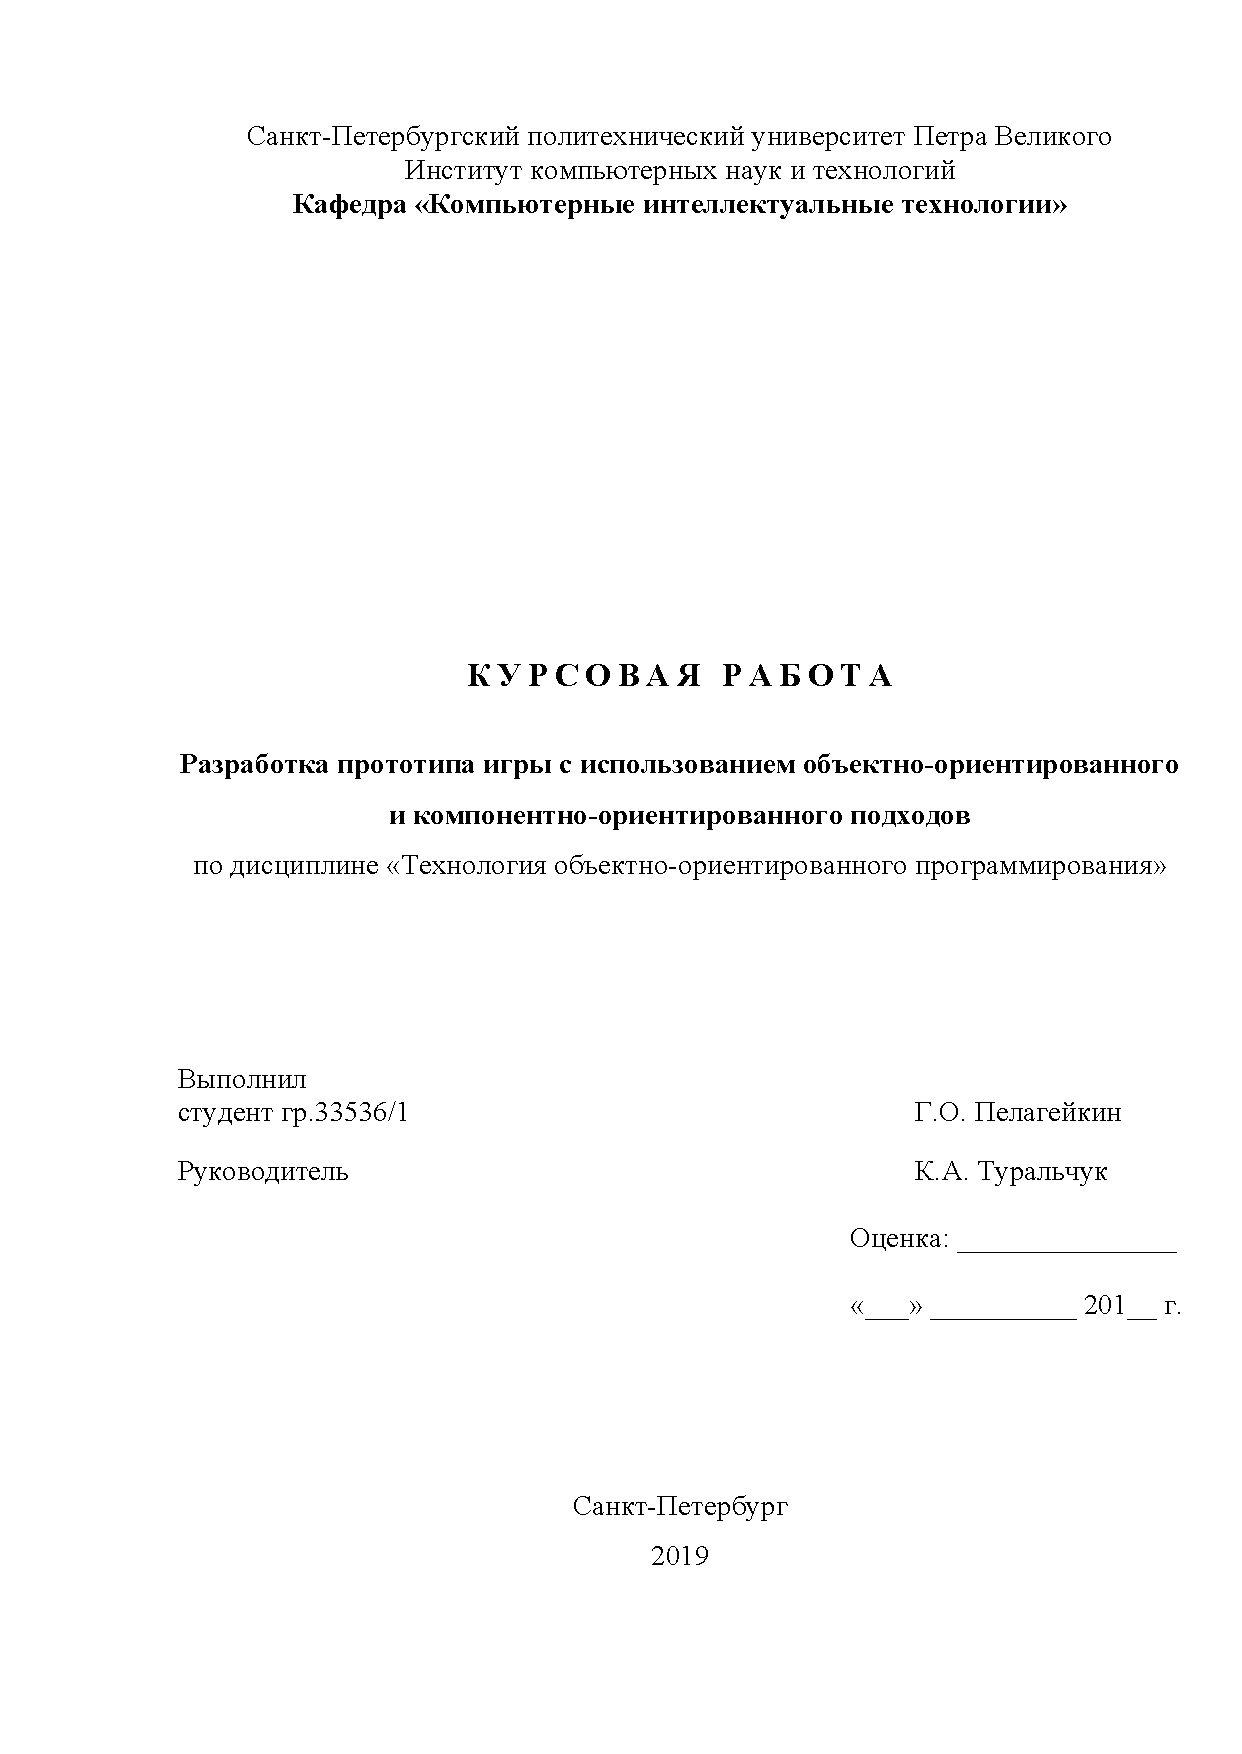
\includepdf{title-page}

	\tableofcontents

	\begin{anonsection}{Введение}
		В данной работе будет рассмотрен процесс создания простой игры.
		В качестве эталона была взята логика игры <<Atomic Bomber>>, реализация выполнена на языке C++ на основе легковесного игрового движка Urho3D.
		В ходе выполнения работы были выполнены следующие задачи:
		\begin{enumerate}
			\item Декомпозиция задачи.
			\item Реализация основных компонентов игры с использованием парадигмы объектно-ориентированного программирование, а также компонентно-ориентированного подхода, средства реализации которого предоставлены движком Urho3D.
			\item Тестирование и отладка приложения.
		\end{enumerate}

	\end{anonsection}

	\begin{section}{Постановка задачи}
		Приведем основные аспекты игровой логики, которые будут реализованы.
		В качестве эталона рассматривалась игровая логика <<Atomic Bomber>> за авторством Luke Allen:

		\begin{enumerate}
			\item Игровой мир двухмерный, вид сбоку.
			\item Нижнюю часть экрана занимает случайно сгенерированный ландшафт, на поверхности которого могут находиться противники.
			\item Игрок управляет самолетом, имеющим постоянную скорость.
			Правая и левые стороны "закольцованы" друг на друга (т.е. пролет через них телепортирует игрока к противоположной границе), вылет за верхнюю границу также невозможен.
			\item Самолет вооружен бомбами, деформирующими ландшафт при столкновении и уничтожающими находящихся в определенном радиусе противников.
			\item При столкновении самолета с ландшафтом уровень перезагружается.
		\end{enumerate}

		\begin{figure}[h]
			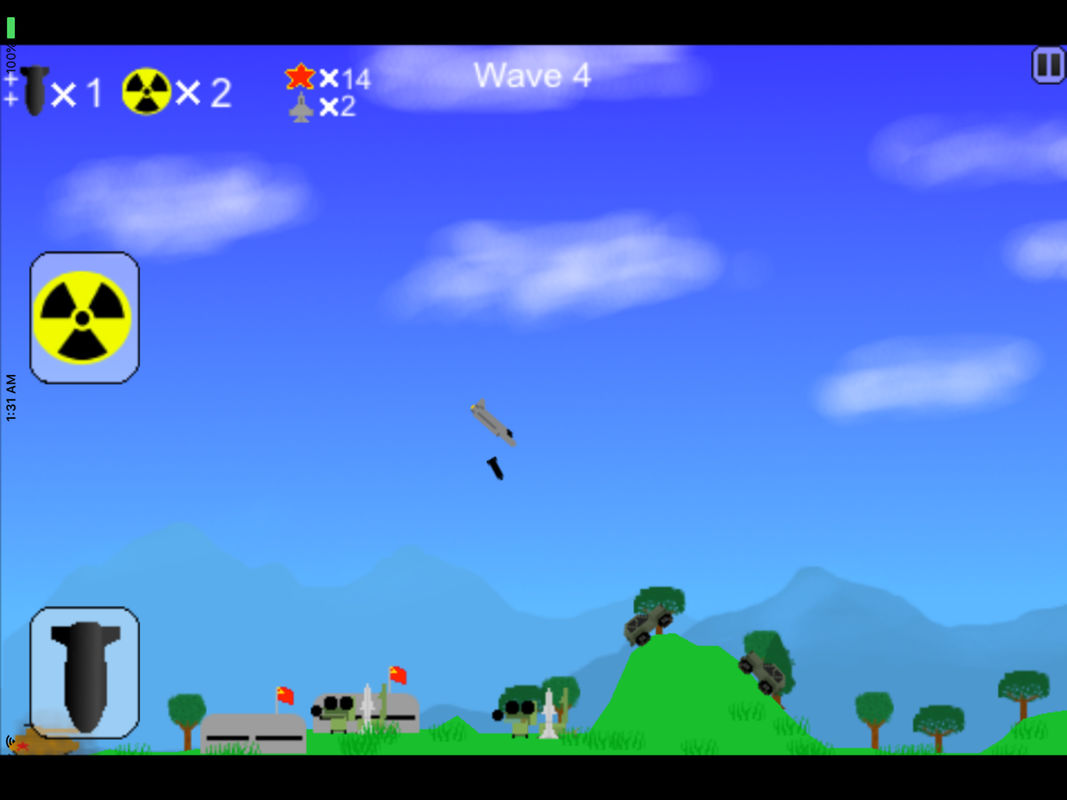
\includegraphics[width=\linewidth]{atomic-bomber}
			\caption{Скриншот игрового процесса <<Alien Bomber>>}
		\end{figure}
	\end{section}

	\begin{section}{Реализация программы}
		\begin{subsection}{Обзор инструментальных средств}
			Разработка программы велась на языке C++ в объектно-ориентированной парадигме программирования.
			Самостоятельная реализация даже самого базового фреймворка для разработки нашего приложения очень трудоемка, поэтому разработка велась с использованием движка Urho3D в качестве фреймворка.
			Он предоставляет такие необходимые компоненты как:
			\begin{enumerate}
				\item Управление жизненным циклом программы, обработка событий ОС.
				\item Компонентно-ориентированная модель для описания объектов в 2D/3D среде (сцене), легковесный визуальный редактор сцен.
				\item Загрузка текстур и других ассетов в различных форматах, рендеринг 2D и 3D графики, вывод звука, рассчет физики, обработка пользовательского ввода и другие важные подисистемы.
			\end{enumerate}

			Компонентно-ориентированный подход к построению сцены позволяет удобно реализовывать логику взаимодействия игровых объектов в 2D/3D пространстве и инкапсулировать отдельные ее аспекты.
			Его реализация в движке Urho3D глубоко интегрирована с объектно-ориентированной парадигмой языка C++ и удачно ее дополняет.

			Также была использована библиотека Signals~\cite{signals} в качестве реализации шаблона проектирования <<Observer>>, предоставляющая функционал сигналов и слотов, похожий на делегаты и события в C#.
		\end{subsection}

		\begin{subsection}{Программная реализация}
			\begin{subsubsection}{Инициализация}
				Входной точкой нашего приложения является класс GameApplication, который регистрируется в движке Urho3D макросом \verb|URHO3D_DEFINE_APPLICATION_MAIN(GameApplication)|.
				В нем производится получение контекста от Urho3D, начальная настройка приложения, вызов регистрации классов компонентов, а также создание и регистрация подсистемы управления игровым состоянием GameSubsystem (в Urho3D подсистемами называются объекты, существующие в единственном экземпляре во всем приложении).

				GameSubsystem предоставляет функционал загрузки, выгрузки и перезагрузки нашего игрового уровня.
				Компоненты на нем, в свою очередь, реагируют на различные события (например, переход на следующий кадр, пользовательский ввод или столкновения), формируя игровой процесс.
			\end{subsubsection}

			\clearpage
			\begin{subsubsection}{Структура уровня}
				Уровень (сцена) представляет собой иерархию объектов (называемых Node) и их компонентов:

				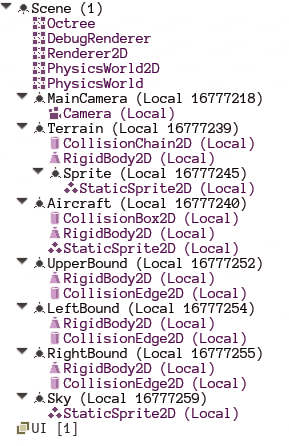
\includegraphics[width=250]{scene}

				\begin{enumerate}
					\item Объект MainCamera в нашем случае является закрепленной на одном месте ортогональной (не перспективной, т.к. наш мир двухмерен) камерой.
					Автоматически масштабируется при запуске для корректного отображения игровой области.
					\item Объект Terrain представляет ландшафт.
					\item Объект Aircraft представляет самолет игрока.
					\item Объект Sky отображает спрайт неба на заднем плане.
					\item Объекты LeftBound, RightBound и UpperBound расположены по краям видимой области и содержат физические коллайдеры, не позволяющие игроку покинуть пределы видимого пространства.
				\end{enumerate}

				Рассмотрим их подробнее.
			\end{subsubsection}

			\begin{subsubsection}{Ландшафт}
				Наиболее комплексная система в нашем приложении, состоит из трех компонентов
				\begin{enumerate}
					\item \verb|TerrainController| предоставляет логическую модель ландшафта, с которой работают другие компоненты.
					\item \verb|TerrainSpriteController| занимается динамической отрисовкой спрайта ландшафта.
					\item \verb|TerrainCollisionShapeController| выполняет динамическое построение физической модели ландшафта для работы столкновений.
				\end{enumerate}

				\verb|TerrainController| содержит карту высот: одномерный массив чисел с плавающей точкой, содержащий высоты в соответствующих точках ландшафта.
				Предоставляет методы для деформации ландшафта (взрыва), перевода координат из относительных координат (например, 0.5 будет серединой ландшафта) в абсолютные (мировые), а также событие об изменени ландшафта, позволяющее подписчикам отреагировать на это изменение.

				В начале игры карта высот генерируется одномерной версией алгоритма MidpointDisplacement, который рекурсивно генерирует случайную высоту в середине заданного промежутка на основании высот краев:
				\inputminted{cpp}{listings/MidpointDisplacement1D.cpp}

				При любых изменениях карты высот вызывается событие \verb|HeightmapUpdated|, позволяющее указанным выше компонентам перерисовать спрайт и перестроить сетку коллизий.
			\end{subsubsection}
		\end{subsection}
	\end{section}


	\printbibliography[title = Список использованных источников]

\end{document}
